\def\year{2021}\relax
%File: formatting-instructions-latex-2021.tex
%release 2021.2
\documentclass[letterpaper]{article} % DO NOT CHANGE THIS
\usepackage{aaai21}  % DO NOT CHANGE THIS
\usepackage{times}  % DO NOT CHANGE THIS
\usepackage{ctex}
\usepackage{helvet} % DO NOT CHANGE THIS
\usepackage{courier}  % DO NOT CHANGE THIS
\usepackage[hyphens]{url}  % DO NOT CHANGE THIS
\usepackage{verbatim}
\usepackage{graphicx} % DO NOT CHANGE THIS
\urlstyle{rm} % DO NOT CHANGE THIS
\def\UrlFont{\rm}  % DO NOT CHANGE THIS
\usepackage{natbib}  % DO NOT CHANGE THIS AND DO NOT ADD ANY OPTIONS TO IT
\usepackage{caption} % DO NOT CHANGE THIS AND DO NOT ADD ANY OPTIONS TO IT
\frenchspacing  % DO NOT CHANGE THIS
\setlength{\pdfpagewidth}{8.5in}  % DO NOT CHANGE THIS
\setlength{\pdfpageheight}{11in}  % DO NOT CHANGE THIS
%\nocopyright
%PDF Info Is REQUIRED.
% For /Author, add all authors within the parentheses, separated by commas. No accents or commands.
% For /Title, add Title in Mixed Case. No accents or commands. Retain the parentheses.
%Leave this
% /Title ()
% Put your actual complete title (no codes, scripts, shortcuts, or LaTeX commands) within the parentheses in mixed case
% Leave the space between \Title and the beginning parenthesis alone
% /Author ()
% Put your actual complete list of authors (no codes, scripts, shortcuts, or LaTeX commands) within the parentheses in mixed case.
% Each author should be only by a comma. If the name contains accents, remove them. If there are any LaTeX commands,
% remove them.

% DISALLOWED PACKAGES
% \usepackage{authblk} -- This package is specifically forbidden
% \usepackage{balance} -- This package is specifically forbidden
% \usepackage{color (if used in text)
% \usepackage{CJK} -- This package is specifically forbidden
% \usepackage{float} -- This package is specifically forbidden
% \usepackage{flushend} -- This package is specifically forbidden
% \usepackage{fontenc} -- This package is specifically forbidden
% \usepackage{fullpage} -- This package is specifically forbidden
% \usepackage{geometry} -- This package is specifically forbidden
% \usepackage{grffile} -- This package is specifically forbidden
% \usepackage{hyperref} -- This package is specifically forbidden
% \usepackage{navigator} -- This package is specifically forbidden
% (or any other package that embeds links such as navigator or hyperref)
% \indentfirst} -- This package is specifically forbidden
% \layout} -- This package is specifically forbidden
% \multicol} -- This package is specifically forbidden
% \nameref} -- This package is specifically forbidden
% \usepackage{savetrees} -- This package is specifically forbidden
% \usepackage{setspace} -- This package is specifically forbidden
% \usepackage{stfloats} -- This package is specifically forbidden
% \usepackage{tabu} -- This package is specifically forbidden
% \usepackage{titlesec} -- This package is specifically forbidden
% \usepackage{tocbibind} -- This package is specifically forbidden
% \usepackage{ulem} -- This package is specifically forbidden
% \usepackage{wrapfig} -- This package is specifically forbidden
% DISALLOWED COMMANDS
% \nocopyright -- Your paper will not be published if you use this command
% \addtolength -- This command may not be used
% \balance -- This command may not be used
% \baselinestretch -- Your paper will not be published if you use this command
% \clearpage -- No page breaks of any kind may be used for the final version of your paper
% \columnsep -- This command may not be used
% \newpage -- No page breaks of any kind may be used for the final version of your paper
% \pagebreak -- No page breaks of any kind may be used for the final version of your paperr
% \pagestyle -- This command may not be used
% \tiny -- This is not an acceptable font size.
% \vspace{- -- No negative value may be used in proximity of a caption, figure, table, section, subsection, subsubsection, or reference
% \vskip{- -- No negative value may be used to alter spacing above or below a caption, figure, table, section, subsection, subsubsection, or reference

\setcounter{secnumdepth}{0} %May be changed to 1 or 2 if section numbers are desired.

% The file aaai21.sty is the style file for AAAI Press
% proceedings, working notes, and technical reports.
%

% Title

% Your title must be in mixed case, not sentence case.
% That means all verbs (including short verbs like be, is, using,and go),
% nouns, adverbs, adjectives should be capitalized, including both words in hyphenated terms, while
% articles, conjunctions, and prepositions are lower case unless they
% directly follow a colon or long dash

\title{ 探索信息奥秘 \quad 机器学习初阶实战 \\	课程报告 }
\author{
    %Authors
    % All authors must be in the same font size and format.
   李思进 2021270901014
    \\
}
\affiliations{
    %Afiliations
    电子科技大学 英才实验学院\\ Yingcai Honors College of UESTC
    %If you have multiple authors and multiple affiliations
    % use superscripts in text and roman font to identify them.
    %For example,

    % Sunil Issar, \textsuperscript{\rm 2}
    % J. Scott Penberthy, \textsuperscript{\rm 3}
    % George Ferguson,\textsuperscript{\rm 4}
    % Hans Guesgen, \textsuperscript{\rm 5}.
    % Note that the comma should be placed BEFORE the superscript for optimum readability

    % email address must be in roman text type, not monospace or sans serif
    sjin.li@std.uestc.edu.cn

    % See more examples next
}
\iffalse
%Example, Single Author, ->> remove \iffalse,\fi and place them surrounding AAAI title to use it
\title{My Publication Title --- Single Author}
\author {
    % Author
    Author Name \\
}

\affiliations{
    Affiliation \\
    Affiliation Line 2 \\
    name@example.com
}
\fi

\iffalse
%Example, Multiple Authors, ->> remove \iffalse,\fi and place them surrounding AAAI title to use it
\title{My Publication Title --- Multiple Authors}
\author {
    % Authors
    First Author Name,\textsuperscript{\rm 1}
    Second Author Name, \textsuperscript{\rm 2}
    Third Author Name \textsuperscript{\rm 1} \\
}
\affiliations {
    % Affiliations
    \textsuperscript{\rm 1} Affiliation 1 \\
    \textsuperscript{\rm 2} Affiliation 2 \\
    firstAuthor@affiliation1.com, secondAuthor@affilation2.com, thirdAuthor@affiliation1.com
}
\fi
\begin{document}

\maketitle

\begin{abstract}
本文总结了机器学习初阶实战课程的主要内容和学习收获,和对机器学习、链路预测、强化学习框架的概述性浅显总结。
\end{abstract}

机器学习初阶实战是学院大一学生的新生项目课程,目的是为了更早的了解行业、了解前沿技术、了解技术中的数学原理……这门课程主要介绍了机器学习的基础知识、图的基础、链路预测的几种方法,到后来的马尔科夫决策过程、强化学习(Reinforcement Learning)基础。

\section{学习与预测}

\subsection{主要内容}
学习与预测主要内容是:使用机器学习对链路进行预测,比如“可能认识的人”的预测,所有的人用图中的一个节点表示。

图在计算机中以一种基础的方式存储起来:邻接矩阵,属于空间占用较大的一种方法,但更加方便理解入门。

目标:给出一张图,这个图中已经有一些边,也许表示“这两个人认识”,要找出没有直接连线的节点,他们也相互认识。即:评估计算两个节点之间的“距离”,“亲密程度”,找出隐含的边。将数据分为训练集和测试集,训练后给出推测结果。

\subsection{不同算法}

\subsubsection{Local Prediction}

\begin{enumerate}
	\item Common neighbors (CN) 
		顾名思义:共同好友、共同邻居,容易理解。
		
		$$s_{x y}^{C N}=|\Gamma(x) \cap \Gamma(y)| \quad $$ $\Gamma(x)$: set of neighbors 
		
	\item Jaccard (JC) 
		CN的演化:
		$$
		s_{x y}^{J C}=\frac{C N}{k_{x}+k_{y}-C N}
		$$
		
		$k$: degree of a node
		不仅考虑了共同好友数量,还考虑了共同好友的占比。
		
	\item Adamic-Adar (AA)
	$$s_{x y}^{A A}=\sum_{z \in \Gamma(x) \cap \Gamma(y)} \frac{1}{\log k_{z}}$$
	
	对于每个共同好友的度进行计算,两者共同好友的度越小,两者对于他就有更高重要性,$s_{x y}^{A A}$也就越大。
	
	\item Preferential attachment (PA)
	
	$$s_{xy}^{PA}=k_x k_y $$
	
	直接计算两者的度。连接更多的节点更有可能形成更多的连接(社交网上遇到社交牛逼症的人了,或者说一个人同时是两个明星的粉丝,两个明星可能就比较相关)
	
	\item ......
\end{enumerate}

\subsubsection{Global Prediction}

\begin{enumerate}
	\item Katz score
	
	计算两个节点之间的路径,随着长度的增长而衰减。
	
	$$ S = \beta A +\beta^2 A^2 + \beta^3 A^3 ... =(I-\beta A)^{-1}-I$$
	
	各种长度的路径带权和,更短的路径影响更大。
	
	\item Hitting time
	
	随机从一个节点走向另一个节点,所需时间的期望值。
	
	\item PageRank
	
	利用指向他的网站数、他指出去的网站数等参数计算两个网站之间的“亲密度”
	
	\item ……

\end{enumerate}




\subsection{一次生动的举例:邻接矩阵乘法的实际含义}、

如果用矩阵$A$表示两个人之间的连线数量,将这个矩阵平方,那么表示经过两个人的情况下能够到达的人的数量。

推广:$A^n$表示经过n个人可以的到达的节点数量。用邻接矩阵表示就是,经过$n$条边能够到达的节点。

\subsection{线性回归}
线性回归是机器学习基础中的核心。

\subsection{算法的AUC}

讨论AUC之前,需要先了解什么是ROC。

ROC(receiver operating characteristic curve)曲线的横坐标是伪阳性率(也叫假正类率,False Positive Rate),纵坐标是真阳性率(真正类率,True Positive Rate),相应的还有真阴性率(真负类率,True Negative Rate)和伪阴性率(假负类率,False Negative Rate)。

而AUC(Area Under Curve)被定义为ROC曲线下的面积。AUC可以衡量二分类模型优劣,表示预测的正例排在负例前面的概率。AUC越接近1,预测效果越好,而AUC若0.5以下还不如随机猜想,但如果换为反预测,就可以优于随机。


\subsection{算法准确性评价:Precision}

引入指标Precition来评价算法的准确性。考虑所有预测的边,按分数值排序。选取其中前$L$ 个。如果和测试集对比后,
其中有 $m $个预测准确,则Precision计算为:
$$Precision = \frac{m}{L}$$

\subsection{插曲:过拟合}

如果测试数据不够大,且模型参数够多,这样训练很多次,最后对于训练过的数据或相似的数据或有很高的准确性,但是如果遇到了一些新的数据,准确率就会降低不少。这种现象叫做过拟合Overfitting。是由于在训练中模型过于与已有数据靠近,甚至学习了一些其它不重要的特征,导致对于其他数据的准确度不够可观。


\subsection{作业}
学习与预测中,我们第一次作业:建立矩阵、数每两个节点之间的common neighbor 的数目、最后print out。
最后的程序在Github Repo 中。同时附带了.exe文件,欢迎尝试。


\section{学习与决策}
\subsection{主要内容}

学习与决策中,我们学习了智能体的概念,和决策的方法,以及一些经典决策算法最后我们通过实践、计算感受了智能体是如何在迭代中利用已知信息不断提升决策水平的。

\subsection{强化学习}

强化学习是一种交互性学习方式,机器玩游戏,通过不断尝试迭代而升级,就先人一样,玩的越多就越熟练。强化学习是机器学习的第三大分支,其框架独特,可以利用其他学习的方法,但其他学习难以刻画强化学习的组件。

四要素:策略、收益信号、状态估值、环境模型。

\subsection{马尔科夫决策过程 Markov Reward Process}

历史是一连串的观察,行动和奖赏。

状态是历史的函数,用来决定即将发生的情况。

未来只与现在状态有关,与历史无关,如果现在状态已经确定,则之前的状态可以被忽略。


\subsection{Bellman Equation}

在本节中,举了“学生决策”的例子。学生可以选择上课或者学习,上课会考砸,而先学习会通过考试从而获得很大的快乐,为了获得更多快乐,需要考虑短期收益和长期收益。

Bellman Equation for MRPs do as well.当前状态变量分为两个部分:直接收益和间接收益。

\begin{center}
	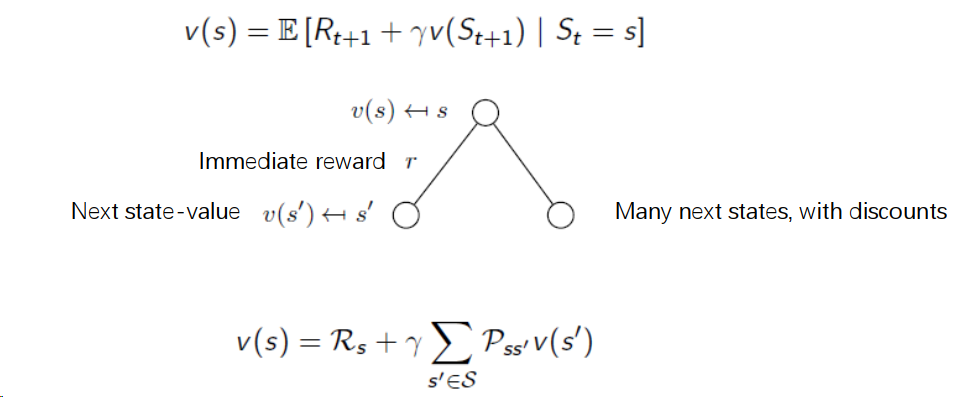
\includegraphics[width=\linewidth]{screenshot003}
\end{center}


\subsection{作业}
学习与决策中,我们有了第二次作业:根据马尔科夫决策过程和一张流向图,设定一个$\gamma$来算出每个点的权值。
下面的计算中$\gamma = 0.5$ 
\begin{center}
	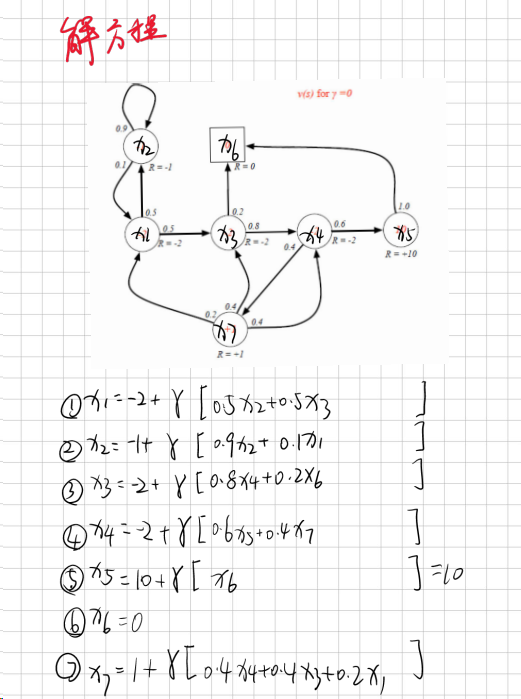
\includegraphics[width=0.9\linewidth]{screenshot001}
\end{center}

\begin{center}
	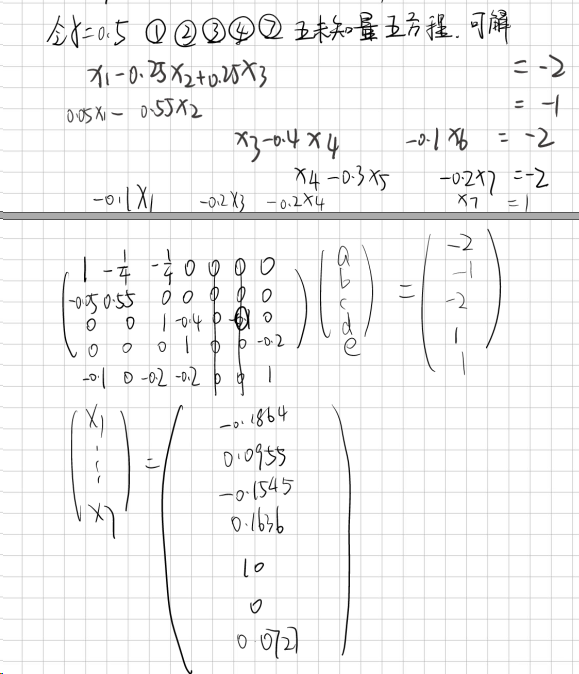
\includegraphics[width=0.9\linewidth]{screenshot002}
\end{center}



\subsection{总结}
学习与决策专题的主要内容是强化学习,而强化学习是一座大山,课程之余我去看了一些Github的仓库,了解到,这里的马尔科夫决策过程和Q-learning 都是强化学习中最基础的算法之一,还有很多更先进的算法,共同筑起了当今社会AI的伟大应用。

强化学习的主要应用场景是竞技类、比赛类AI,通过自己试错,自己演化的方式提升竞技能力,十分方便。这些数学公式和描述就能制作出如此有趣的玩具,实在是神奇,而这些魔法一样的玩具背后都是严密的数学推导,又能让我更加重视数理能力,同时通过Project的尝试锻炼了实践能力,最后被它深深吸引。

\section{总结}

本次新生项目课程让我收获良多,从最开始的链路预测,到最后的马尔科夫决策,讲得深入浅出,节奏稳当,也注重数学基础和底层逻辑,重视推导过程,降低了我理解的难度。



\section{Notes \& Source}

Project Source Link (Github):
\url{https://github.com/Sjin-Lee/UESTC_Freshman_Project}




\begin{thebibliography}{100}%此处数字为最多可添加的参考文献数量
	%\bibitem{article1}This is reference.%title author journal data pages	
	\bibitem{teacher}一个讲义。
	\url{https://www.cis.upenn.edu/~cis519/fall2015/lectures/14_ReinforcementLearning.pdf} 
	
	\bibitem{AnotherOne}机器学习相关知识。
	
	\url{https://github.com/sckangz/DeepLearning-500-questions}
	
	\bibitem{citekey}强化学习的一个仓库。
	
	\url{https://github.com/dennybritz/reinforcement-learning}
	
	\bibitem{aaai}报告排版模板来自AAAI Author Kit. 
	
	\url{https://www.aaai.org/}
	
\end{thebibliography}

\end{document}
